\documentclass{beamer}

\usepackage{smartdiagram}

\usetheme{default}
\usecolortheme{default}
\usefonttheme{default}

\title{Low-Level Network Programming and Operating Systems Development}
\author{Jacob Bates}
\institute{Da Vinci Science High School}

\begin{document}

\section{Title}

    \begin{frame}
        \titlepage
    \end{frame}

\section{Project}

    \begin{frame}{Project}
        \begin{itemize}
            \item Involved with Low-Level Programming
            \item Interested in Networking
        \end{itemize}
        \rule{0.5\textwidth}{0.5pt}\\
        \begin{itemize}
            \item Operating System for IA-32
            \item Written in C
            \item Network Driver
            \item Network Stack
            \item TFTP Storage Server
        \end{itemize}
    \end{frame}

\section{Hardware}

    \begin{frame}{Network Adaptor - Realtek RTL8139}
        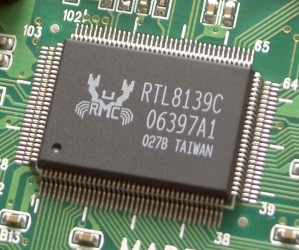
\includegraphics[height=125pt]{Realtek_RTL8139C.jpg} \\
        \rule{0.5\textwidth}{0.5pt} \\
        \begin{itemize}
            \item Older Chip (1999)
            \begin{itemize}
                \item Easier to Program
                \item Widely Used
                \item Inexpensive
            \end{itemize}
            \item PCI Card
        \end{itemize}
    \end{frame}

\section{Standards}

    \begin{frame}{The OSI Model}
        \smartdiagramset{
            description font= \scriptsize,
            descriptive items y sep=1.15
        }
        \smartdiagram[priority descriptive diagram]{
            {\textbf{Physical} (Ethernet): responsible for encoding data onto the physical link},
            {\textbf{Data-Link} (MAC, LLC): provides data transfer across a link (local network)},
            {\textbf{Network} (IPv4): enables communication across multiple data links (wide network)},
            {\textbf{Transport} (UDP, TCP): provides abstractions for conveying arbitrary data},
            {\textbf{Session} (TCP): provides a "dialogue" model},
            {\textbf{Presentation/Application} (TFTP, HTTP): highest-level communication protocol, specific to programs}
        }
    \end{frame}

\section{Implementation}

    \begin{frame}{Implementation}
        \smartdiagramset{
            back arrow disabled=true
        }
        \begin{block}{Internet Protocol Handler}
            \smartdiagram[flow diagram:horizontal]{
                Copy Packet to Buffer, Validate Destination \& Checksum, Cache HW Address, Call Higher Protocol
            }
        \end{block}
        \begin{block}{Internet Protocol Send Routine}
            \smartdiagram[flow diagram:horizontal]{
                Frame Payload \& Length, Compute Checksum, Query HW Address, Call Driver
            }
        \end{block}
    \end{frame}

\end{document}
